\subsubsection{Installation d'une image précompilée}

Pour premier tester l'Installation de linux sur la carte de développement, j'ai utilisé une image de la distribution Ubuntu fournie par le fabriquant 96Boards disponible sur leur site. Cette image se présente sous la forme d'une archive au format \texttt{.tar.gz}. Elle contient à la fois le \gls{bootloader}, le noyau Linux, et le système de fichier. Cette image (\texttt{system.img}) peut alors être gravée (ou \textit{flashée}) sur une carte micro SD. 

Depuis un terminal, en se déplaçant dans le dossier de l'archive extraite, on exécute la commande suivante : 
\begin{lstlisting}[style=command]
$ sudo dd if=system.img of=/dev/XXX bs=4M oflag=sync status=noxfer
\end{lstlisting}

\begin{center}
    \color{red}
    EXPLIQUER CE QUE FAIT CETTE COMMANDE \\
    Aussi dire en quoi on s'en servira dans des scripts afin d'accélérer le développement.
\end{center}


\subsubsection{Compilation de Linux depuis le code source}\label{sec:compilation-linux-source}

Afin d'utiliser une version de Linux différente de la version précompilé par le fabriquant de la carte de développement, il faut se premièrement se procurer le code source du noyau Linux. Celui-ci est disponible sur un dépôt de code \gls{git} hébergé par GitHub. Il est disponible a l'adresse \texttt{https://github.com/torvalds/linux}, sous le profile du créateur de Linux : Linus Torvalds. Durant mon stage j'étais libre d'utiliser le logiciel de gestion de version de mon choix, j'ai donc principalement utilisé \textit{git} en ligne de commande et j'ai parfois utilisé un client git nommé \textit{GitKraken} afin plus facilement explorer les anciens commits de certains projets comme \litmus.

Une fois le code source du noyau téléchargé, et en se déplaçant dans le dossier \texttt{linux} depuis un terminal, on peu alors procédé a la compilation. Pour mes premiers essais j'ai premièrement décidé de compiler Linux pour une machine virtuelle que je ferai tourner sur ma machine de travail.

Le noyau Linux est un programme ayant une compilation basée sur la configuration : cela signifie que certaines parties du code peuvent rajouter ou omises par le simple biais d'une fichier de configuration. Ce configuration se présente sous la forme d'un fichier \texttt{.config} qui doit être créé à la racine du noyau. Pour créer ce fichier, des utilitaires sont mise a notre disposition dans le noyau :
\begin{itemize}
    \item \texttt{make defconfig} : cet outil est utilisé pour générer une configuration pas défaut. Ici l'architecture de la machine qui réalise la compilation sera sélectionnée. Dans mon cas, éxécuter cette commande créer un fichier de configuration basé sur la config \texttt{'x86\_64\_defconfig'}.
    \item \texttt{make menuconfig} : cet outil permet d'éditer la configuration actuelle du fichier \texttt{.config} via une interface graphique. Ce menu permet aussi de rechercher des paramètres, de voir leur description et d'enregistrer différentes configurations.
\end{itemize}

\begin{figure}[H]
    \centering
    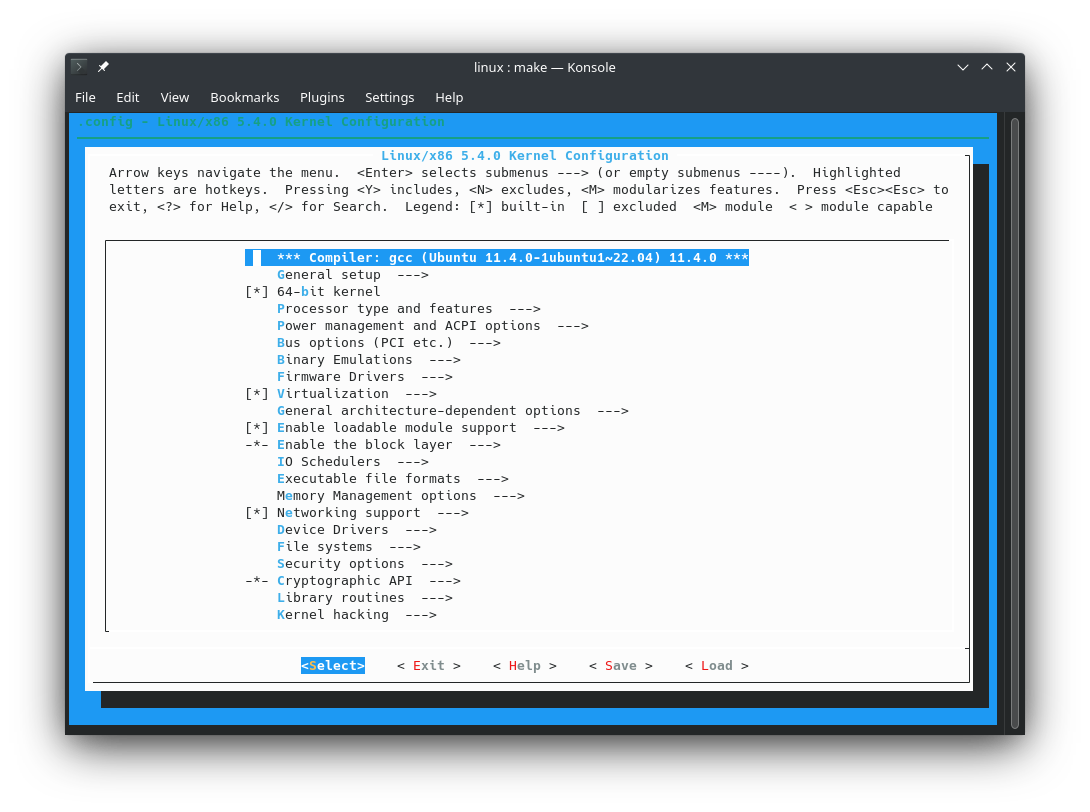
\includegraphics[width=0.65\paperwidth]{Images/make menuconfig.png}
    \caption{Interface de configuration du noyau}
\end{figure}

Une fois la configuration crée, nous pouvons passer à la compilation du noyau. Linux utilise l'utilitaire de compilation \textit{GNU Make} : il permet l'automatisation de la compilation, la gestion des dépendances et gère la personnalisation de la compilation de chaque dossier. Ces règles sont alors dictés par des fichiers \texttt{MakeFile} présent dans chaque dossier contenant des fichiers à compiler du projet.

Note : chaque distribution Linux possède un ensemble différent de programmes préinstallés, il faudra alors peut-être installer des programmes nécessaires a la compilation. Par exemple, installer \texttt{libelf-dev} "une bibliothèque partagée qui permet de lire et écrire des fichiers ELD à un niveau élevé"\footnote{d'après la description sur packages.debian.org/fr/sid/libelf-dev}. 


\vspace{20pt}
Ou est le code source linux ? Expliqué que j'étais déjà familié avec git et github pour des projets persos et tout.

Comment changer de version du code cloné. 

comment modifier quels modules sont chargés lors de la compilation de linux, interface graphique <-> fichier de config.
\subsubsection{Compilation croisée}

Toolchain : qu'est ce que c'est, de quoi elle est constituée ? Expliquer que l'on compile sur du x86 mais qu'on veut compiler pour du ARMv8xxx.

Variables d'environement? Qu'est ce que c'est sous linux, comparer a des 

Réalisation de scripts linux pour accélérer le développement. Que doit on charger pour charger le nouveau code compilé ?

Copy de l'image du noyau pour faire encore plus rapide.

